\documentclass[12pt]{article}
\usepackage[utf8]{inputenc}
\usepackage{float}
\usepackage{amsmath}
\usepackage{fancyvrb}
\usepackage{graphicx}

\usepackage[hmargin=3cm,vmargin=6.0cm]{geometry}
%\topmargin=0cm
\topmargin=-2cm
\addtolength{\textheight}{6.5cm}
\addtolength{\textwidth}{2.0cm}
%\setlength{\leftmargin}{-5cm}
\setlength{\oddsidemargin}{0.0cm}
\setlength{\evensidemargin}{0.0cm}


\begin{document}
\section*{Student Information}
Full Name: Batuhan Akçan\\
Id Number: 2580181
\section*{Answer 1}
\subsection*{a)}
For blue:\\
$P(1) = 1/6, \; P(2) = 1/6, \; P(3)=1/6, \; P(4)=1/6, \; P(5)=1/6, \; P(6)=1/6.$\vspace{0.1cm}\\
$E(X) = \Sigma \; x P(x) = 1\cdot 1/6 + 2 \cdot 1/6 + 3 \cdot 1/6 + 4 \cdot 1/6 + 5 \cdot 1/6 + 6\cdot 1/6 = 3.5.$\vspace{0.1cm}\\
For yellow:\\
$P(1) = 3/8, \; P(3)=3/8, \; P(4)=1/8, P(8)=1/8.$\vspace{0.1cm}\\
$ E(X) = 1\cdot 3/8 + 3\cdot 3/8 + 4\cdot 1/8 + 8\cdot 1/8  = 3.$\vspace{0.1cm}\\
For red:\\
$P(2) = 1/2, \; P(3)=1/5, \; P(4)=1/5, P(6)=1/10.$\vspace{0.1cm}\\
$ E(X) = 2\cdot 1/2 + 3\cdot 1/5 + 4\cdot 1/5 + 6\cdot 1/10  = 3.$
\subsection*{b)}
I would prefer rolling three blue dices because:\vspace{0.1cm}\\
Expected total value of rolling a single dice of each colors:  $E_{blue}(X) + E_{yellow}(X) + E_{red}(X) = 9.5.$\\
Expected total value of rolling 3 blue dices: $E_{blue}(X) \cdot 3 = 10.5.$\\
$10.5 > 9.5.$
\subsection*{c)}
Expected total value of rolling a single dice of each colors would change to 14.5. That's why, I would choose rolling a single dice of each colors.\vspace{0.1cm}\\
$E_{blue}(X) + 8 + E_{red}(X) = 14.5 \; > \; E_{blue}(X) \cdot 3 = 10.5.$
\subsection*{d)}
$V$: value of the dice is 3\\
$R$: the rolled dice is red\\
The question is asking us to find $P(R|V)$ , which is equal to $\frac{P(V|R)\cdot P(R)}{P(V)}$.\\
$P(V|R) = 2/10 = 1/5.$\\
$P(R) = 1/3.$\\
$P(V) = 6/24 = 1/4.$\; (total number of 3's divided by total number of values)\\
Hence, \;$ P(R|V) = \frac{\frac{1}{5}\cdot \frac{1}{3}}{\frac{1}{4}} \approx 0.2667. $
\subsection*{e)}
1 from blue, 4 from yellow: $P_{blue}(1) \cdot P_{yellow}(4) = 1/6 \cdot 1/8 = 1/48.$\vspace{0.1cm}\\
2 from blue, 3 from yellow: $P_{blue}(2) \cdot P_{yellow}(3) = 1/6 \cdot 3/8 = 3/48.$\vspace{0.1cm}\\
4 from blue, 1 from yellow: $P_{blue}(4) \cdot P_{yellow}(1) = 1/6 \cdot 3/8 = 3/48.$\vspace{0.1cm}\\
Result: $1/48 + 3/48 + 3/48 = 7/48 \approx 0.1458.$
\section*{Answer 2}
\subsection*{a)}
I will use Poisson approximation of Binomial Distribution in this part.\\
$n=80, \; p=0.025 \; \rightarrow \lambda = n \cdot p = 2.$\\
$P\{X>=4\} = 1 - F(3) = 1 - 0.857 = 0.143.$
\subsection*{b)}
I will use Poisson approximation of Binomial Distribution for Company A, Binomial Distribution for Company B.\vspace{0.1cm}\\
$A$: company A offers a discount\\
$B$: company B offers a discount\\
$C$: a discount is offered\vspace{0.1cm}\\
We will try to find $P_C\{X>=1\}$ which means at least 1 discount is offered (assuming that we can buy a phone when at least 1 discount is offered).\vspace{0.1cm}\\
$ P_A\{X>=1\} $ means that at least 1 discount is offered by company $A$. Since $\lambda = 2$ for one day for $A$ (found in the previous part), for two days, $\lambda = 4$. $ P_A\{X>=1\} = 1 - F_A(0) = 0.982. $\vspace{0.1cm}\\
$ P_B\{X>=1\} $ means that at least 1 discount is offered by company $B$. Since we are doing the experiment for 2 days, $n=2.$ Also, $p=0.1$ which is given. $ P_B\{X>=1\} = 1 - F_B(0) = 0.190. $\vspace{0.1cm}\\
With $\lambda = 4$, $ P_A\{X=0\} = 0.018. $\vspace{0.1cm}\\
With $n=2$ and $p=0.1$, $ P_B\{X=0\} = 0.81. $\vspace{0.1cm}\\
Hence, the result is:\\
$P_C\{X>=1\} = P_A\{X>=1\} \cdot P_B\{X=0\} + P_A\{X=0\} \cdot P_B\{X>=1\} \\ = 0.982 \cdot 0.81 + 0.190 \cdot 0.018 = 0.79884. $
\section*{Answer 3}
Average total value for the first option: 9.586\\
Average total value for the second option: 10.612\\
Percentage of the cases where the total value of the second option is greater than the first option: 56.4
\subsection*{My code:}
\begin{Verbatim}[tabsize=4]
blue = [1,2,3,4,5,6];
yellow = [1,1,1,3,3,3,4,8];
red = [2,2,2,2,2,3,3,4,4,6];

idx_b = randi (numel (blue), 1000, 1);
idx_y = randi (numel (yellow), 1000, 1);
idx_r = randi (numel (red), 1000, 1);

values_b = blue (idx_b);
values_y = yellow (idx_y);
values_r = red (idx_r);

values1 = [];

i = 1;
while (i <= 1000)
	values1(i) = values_b(i) + values_y(i) + values_r(i);
	i += 1;
endwhile

mean1 = mean (values1);   # answer of the 1st question

idx_b_1 = randi (numel (blue), 1000, 1);
idx_b_2 = randi (numel (blue), 1000, 1);
idx_b_3 = randi (numel (blue), 1000, 1);

values_b_1 = blue (idx_b_1);
values_b_2 = blue (idx_b_2);
values_b_3 = blue (idx_b_3);

values2 = [];

i = 1;
while (i <= 1000)
	values2(i) = values_b_1(i) + values_b_2(i) + values_b_3(i);
	i += 1;
endwhile

mean2 = mean (values2);   # answer of the 2nd question



i = 1;
total = 0;
while (i <= 1000)
	if (values2(i) > values1(i))
		total += 1;
	endif
	i += 1;
endwhile

percentage = total / 10;   # answer of the 3rd question
\end{Verbatim}

\vspace{3cm}
\subsection*{The screenshot:}
\begin{figure}[htbp]
\centerline{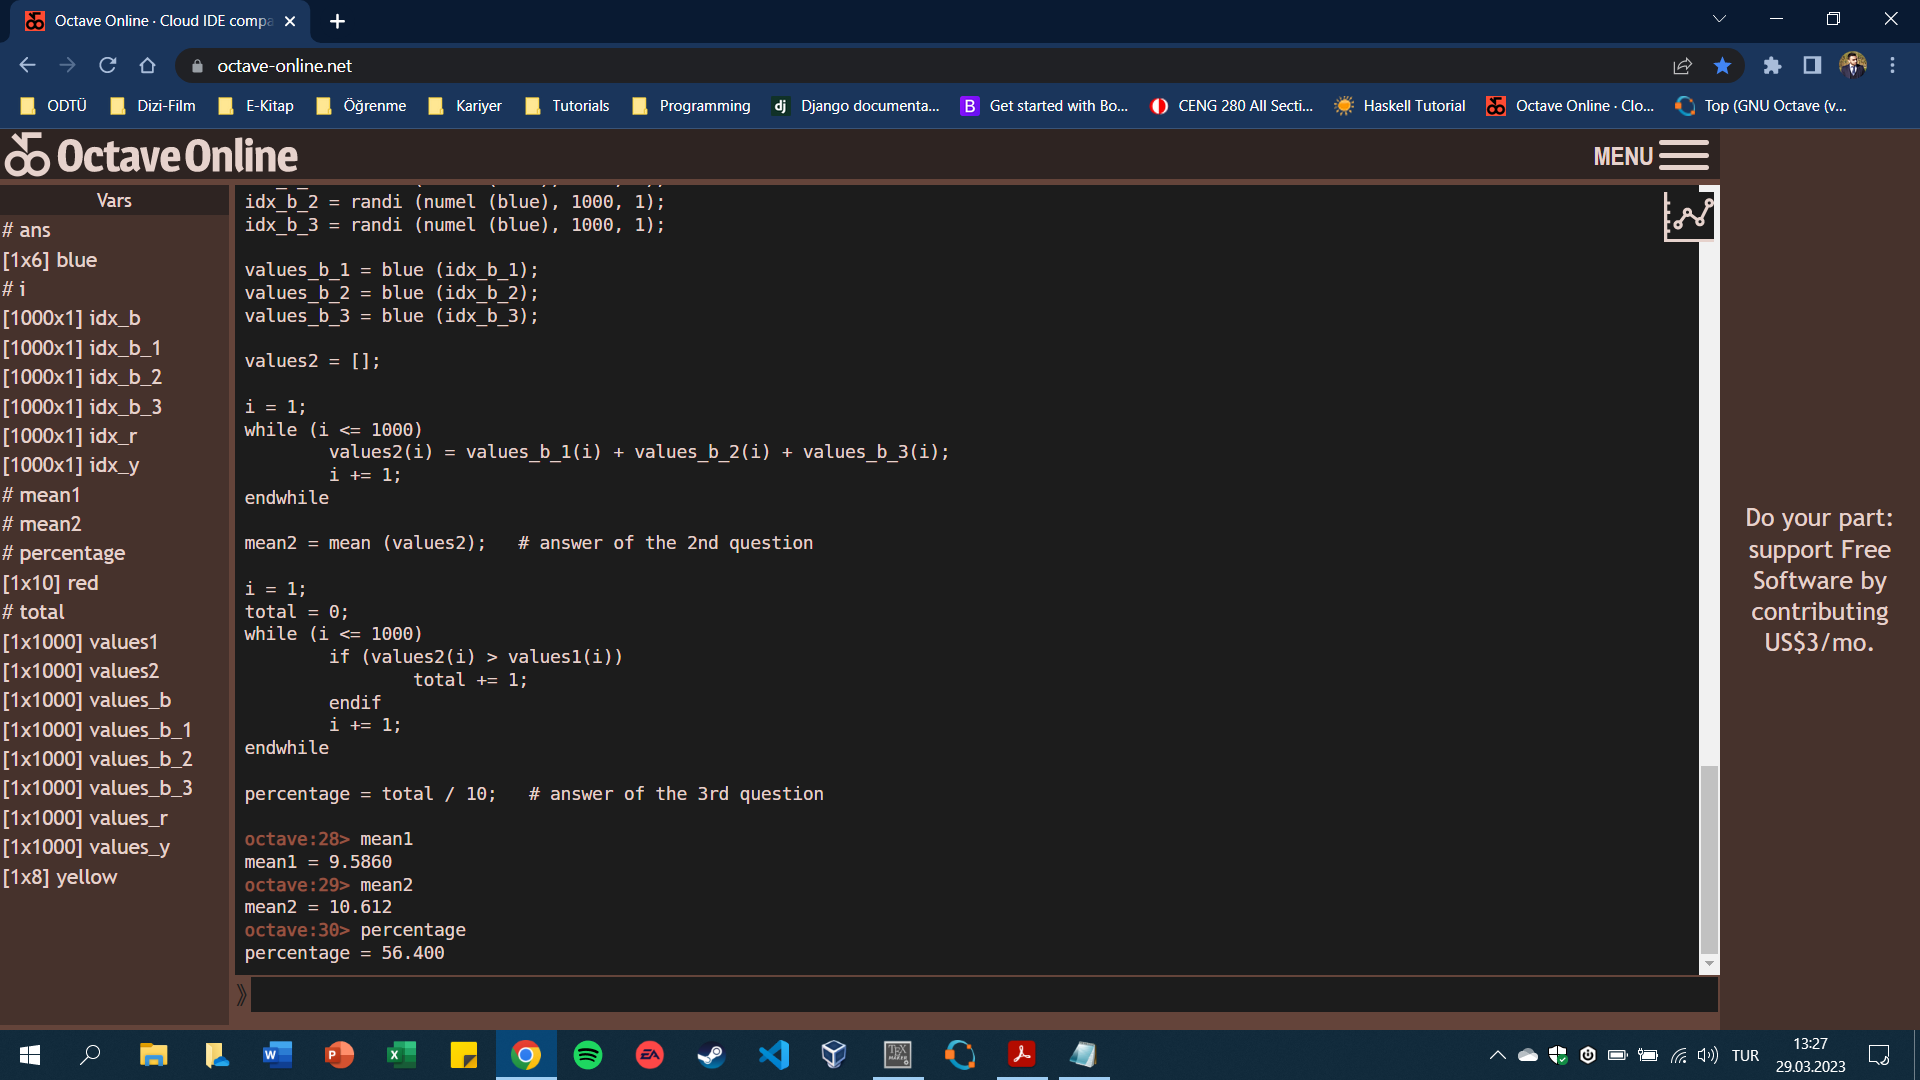
\includegraphics[scale=.5]{222.png}}
\end{figure}

\vspace{3cm}
\subsection*{Comments:}
The results $9.586$ and $10.612$ are approximately equal to the results I have found in Q1b, that are $9.50$ and $10.50$.\\
The percentage is greater than $50\%$, which is what I expected because $10.612 > 9.586$. If the percentage had been $50\%$, then the resultant mean values would have been nearly equal to each other.




\end{document}